\documentclass[runningheads]{llncs}
\usepackage[T1]{fontenc}
\usepackage{graphicx}
\usepackage{booktabs}
\usepackage[misc]{ifsym}
\newcommand{\corr}{(\Letter)}

% custom imports
\usepackage{mwe}
\usepackage{amsfonts}
\usepackage{amsmath}
\usepackage{amssymb}
\usepackage{bm}
\usepackage{mathtools}

\newcommand{\model}{OPAL}
% ======= Table=======
\usepackage{xcolor}
\usepackage{multirow}
\usepackage[normalem]{ulem}
\newcommand{\first}[1]{\textcolor{red}{#1}}
\newcommand{\second}[1]{\textcolor{orange}{#1}}
\newcommand{\third}[1]{\textcolor{blue}{#1}}
\newcommand{\fourth}[1]{\textbf{#1}}
\newcommand{\fifth}[1]{\uline{#1}}

\def\sG{{\mathcal{G}}}
\def\sV{{\mathcal{V}}}
\def\sE{{\mathcal{E}}}
\def\sY{{\mathcal{Y}}}
\def\sL{{\mathcal{L}}}
\def\sQ{{\mathcal{Q}}}
\def\sP{{\mathcal{P}}}
\def\sH{{\mathcal{H}}}

\def\dP{{\mathbb{P}}}
\def\real{{\mathbb{R}}}

\def\mA{{\mathbf{A}}}
\def\mB{{\mathbf{B}}}
\def\mD{{\mathbf{D}}}
\def\mE{{\mathbf{E}}}
\def\mF{{\mathbf{F}}}
\def\mH{{\mathbf{H}}}
\def\mI{{\mathbf{I}}}
\def\mL{{\mathbf{L}}}
\def\mP{{\mathbf{P}}}
\def\mQ{{\mathbf{Q}}}
\def\mR{{\mathbf{R}}}
\def\mW{{\mathbf{W}}}
\def\mX{{\mathbf{X}}}
\def\mY{{\mathbf{Y}}}
\def\mSigma{{\bm{\Sigma}}}

\def\one{{\mathbf{1}}}

\DeclareMathOperator{\Law}{Law}
\DeclareMathOperator{\MMD}{MMD}
\DeclareMathOperator{\Sink}{Sink}
\DeclareMathOperator{\OT}{OT}
\DeclareMathOperator{\CE}{CE}
\DeclareMathOperator{\tr}{tr}
\DeclareMathOperator{\diag}{diag}
\DeclareMathOperator{\rank}{rank}
\DeclareMathOperator{\Lip}{Lip}

\begin{document}

\title{Structural Domain Adaptation via Operator-Level Alignment}
\author{Author information scrubbed for double-blind reviewing}
\maketitle

\begin{abstract}


Unsupervised graph domain adaptation (UGDA) is challenging because distribution shift affects not only node features but also the graph propagation mechanism itself. Existing methods mainly align node embeddings, modify topology, or regularize spectral statistics, but these mechanisms do not directly prevent structure-induced shift from reappearing after each message-passing step. We propose \textbf{\model}, a filter-centric UGDA framework that aligns \emph{realized graph filters} across domains. \model\ learns a shared feature encoder together with domain-specific graph filters that are reused across layers. The filters are aligned through the response laws they induce on a reference distribution that approximates the feature distribution. Theoretically, we extend Optimal-Transport-based domain adaptation bounds to propagated representations and show that target risk is controlled by a feature-alignment term together with an operator-response term that captures mismatch between the realized propagation operators. Practically, \model\ proposes a filter-response alignment paradigm along with smoothness constraints that arise directly from the theory. The resulting model aligns both semantic representations and structural propagation behavior without graph matching or expensive eigenvalue decomposition, while showing competitive performance with state-of-the-art UGDA baselines.
\end{abstract}

% We analyze the effect of the effect of the different components in the shift bound and empirically show the following properties
% 1) Alignment is beneficial only done up to a certain value ~ often determined by the in-domain distribution shift. Above this value, further alignment often hurts performance. Meaning that there is part of the shift that is beneficial for target generalizability and part that is harmful.
% 2) We show that the operator-response term is more important than the feature-alignment term with respect to the effect it has on the target performance. The MMD discrepancy increment introduced by the message passing at one step is often more than 5x the shift introduced by the feature distribution shift. 

%%%%%%%%%%%%%%%%%%%%%%%%%%%%%%%%%%%%%%%%%%%%%%%%%%%%%%%%%%%%%%%%%%%%%%
\section{Introduction}

Graph-structured data arise in a wide range of domains, including citation networks, molecular structures, recommender systems, and social networks. Graph Neural Networks (GNNs) have become the defacto framework for learning from such relational data by combining node attributes with the underlying graph topology through message passing \cite{recsys,graph_tasks1,graph_tasks2,gcn}. This paradigm enables models to exploit dependencies betweein entities and has led to strong performance across many graph-based tasks. However, most GNN models require substantial labeled data to generalize effectively. In many real-world settings, obtaining labels is expensive or impractical. For instance, labeling molecular properties often requires costly simulations or laboratory experiments \cite{material_science,drug_discovery}. These limitations motivate methods that can transfer knowledge across related graph domains.


Domain adaptation addresses this challenge by transferring predictive knowledge from a labeled \emph{source} domain to an unlabeled \emph{target} domain. In graph settings this problem is known as \emph{unsupervised graph domain adaptation} (UGDA), where the goal is to train a model on a labeled source graph and generalize it to an unlabeled target graph that shares the same label space. The difficulty, compared with standard unsupervised domain adaptation, is that the distribution shift is not only semantic but also structural: changing the graph changes message passing, and changing message passing changes the learned representation \cite{gnn_stability}. Consequently, models trained on one graph domain often suffer performance degradation when applied to another, where both node attributes and connectivity patterns may differ.

A natural language for structural shift is graph signal processing. A graph neural network layer can be written in terms of a graph shift operator and a graph filter, whose effect is determined by its frequency response evaluated on the spectrum of the underlying graph \cite{shuman2013emerging,defferrard2016convolutional,gnn_stability}. This viewpoint has already been productive in UGDA. SpecReg cross-pollinates OT-based domain adaptation bounds with graph filter theory and shows that graph transferability is tied to spectral smoothness and maximum frequency response \cite{specreg}, while DGSDA disentangles attribute shift from topology shift and aligns spectral filters across domains \cite{dgsda}. More recent methods such as A2GNN and TDSS similarly highlight that transfer performance depends strongly on how propagation is performed on the source and target graphs \cite{a2gnn,tdss}. Recent benchmarking work further shows that UGDA behavior is strongly scenario-dependent and that structural shift becomes increasingly important as the domain gap grows \cite{pygda}.

Unlike feature shift, which enters the model at the input features, structural shift is reintroduced every time message passing is applied. This makes it inherently architecture-dependent. In our view, the relevant object is therefore not only the spectral response but the realized graph filter
\[
\mR_D = S_{\theta_D}(\widehat{\mA}_D),
\]
obtained by instantiating a response on a domain-specific graph operator. The spectral response is effectively fixed for standard GNN backbones \cite{gcn,dane,udagcn}, prescribed by a simple polynomial rule in propagation-based methods \cite{a2gnn}, and fully learnable in spectral methods \cite{dgsda}. Even if the source and target hidden-feature distributions are well aligned, applying different realized filters can still reintroduce discrepancy. Since the same realized filter is reused at every message-passing layer in our model, any residual structural mismatch is repeatedly applied throughout the network. We therefore aim to align the \emph{operator action} of the realized filters on the feature distributions that actually arise during training, rather than align spectral responses alone.

To address this challenge, we introduce \textbf{OPAL} (\emph{Operator-Level Alignment for Graph Domain Adaptation}), a framework that aligns structural propagation behavior across domains by directly comparing their realized graph filters. \model\ learns a shared feature encoder and a shared classifier, together with domain-specific graph filters that remain fixed across layers. Feature alignment is performed on the shared latent feature space, while filter alignment is performed by sampling a reference distribution that is representative of the feature distribution, propagating it through the domain-specific realized filters, and aligning the resulting response laws. This yields a simple objective that stays close to the OT-based transfer bound while remaining easy to optimize. It also removes the need for graph matching and avoids eigendecomposition in the practical method, because alignment is performed at the level of the learned propagation operators rather than directly on graph structure.

Our contributions are threefold. First, we formulate structural adaptation at the level of realized graph filters and show that the OT-based graph transfer bound naturally decomposes into a feature term and an operator-response term. Second, we derive a practical alignment objective that compares realized filters through the response distributions they induce on a shared feature-supported reference law. Third, we turn these observations into a simple UGDA method that combines source supervision, latent feature alignment, and a Lipschitz-regularized reference-based filter alignment.

%%%%%%%%%%%%%%%%%%%%%%%%%%%%%%%%%%%%%%%%%%%%%%%%%%%%%%%%%%%%%%%%%%%%%%
\section{Related Work}

\paragraph{Benchmarking and taxonomy.}
Recent benchmarking work shows that UGDA performance varies substantially across datasets and transfer scenarios, and that structural shift becomes increasingly important as the domain gap grows \cite{pygda}. This observation is consistent with the way recent graph adaptation papers organize the field: some methods mainly target node representations, some modify graph structure, and others focus on propagation or spectral behavior. Following this view, we group the most relevant UGDA methods into three families: embedding-alignment methods, structure-aware adaptation methods, and propagation- or spectral-based methods.

\paragraph{Embedding alignment methods.}
Early UGDA methods mostly follow the standard domain adaptation pipeline of learning domain-invariant node representations. DANE learns transferable node embeddings with a shared GCN encoder and adversarial alignment across networks \cite{dane}. AdaGCN extends adversarial adaptation with graph convolution to transfer class information across source and target graphs \cite{adagcn}. UDAGCN combines graph representation learning with domain adaptation by jointly modeling local and global consistency, while GRADE introduces a graph subtree discrepancy to measure graph distribution shift and align cross-network representations \cite{udagcn,grade}. These methods are effective when node-level semantic discrepancy is the dominant challenge, but they largely treat propagation as part of the encoder and do not explicitly isolate the mismatch introduced by domain-specific message passing. In contrast, \model\ keeps a shared feature encoder but adds a separate alignment mechanism at the level of the learned propagation operators.

\paragraph{Structure-aware adaptation methods.}
A second line of work addresses graph-specific shift more directly by modifying or reweighting structure. StruRW identifies \emph{conditional structure shift} and proposes structural reweighting to correct it through edge-weight recalibration \cite{stru_rw}. PairAlign further targets conditional structure shift together with label shift by combining pairwise edge reweighting and class-balance adjustment \cite{pair_align}. JHGDA studies shifts in hierarchical graph structure and aggregates discrepancy across multiple hierarchy levels, while KBL introduces a knowledge-bridge mechanism to transfer knowledge through an auxiliary bridged graph and a knowledge-enhanced posterior \cite{jhgda,kbl}. These methods explicitly exploit graph structure and often improve over embedding-only alignment under larger structural shifts, but they do so by changing graph interactions, adding hierarchical graph modules, or introducing extra transfer graphs rather than aligning the learned propagation operators themselves. Compared with these approaches, \model\ does not alter graph topology or require graph matching; instead, it learns domain-specific filters and aligns their induced behavior directly.

\paragraph{Propagation- and spectral-based methods.}
A closely related family of methods emphasizes propagation and spectral behavior. A2GNN argues that propagation itself is the key factor in graph adaptation and improves transfer by using asymmetric propagation depth across source and target branches \cite{a2gnn}. TDSS smooths the target graph directly to reduce structural inconsistency before adaptation \cite{tdss}. SpecReg derives graph-specific OT-based transfer bounds and regularizes spectral smoothness and maximum frequency response, while DGSDA disentangles attribute and topology shift and aligns spectral filters across domains \cite{specreg,dgsda}. These methods are closest in spirit to our work because they recognize that graph transfer depends on how information is propagated, not only on the final embeddings. Our method differs in the alignment target: instead of modifying the graph, changing propagation depth, or aligning spectral responses, \model\ learns domain-specific realized graph filters and aligns them directly through the response laws they induce on a shared reference distribution supported by the learned features.

\paragraph{Position of our method.}
Compared with embedding-alignment methods, \model\ explicitly models the structural part of the transfer gap. Compared with structure-editing methods such as StruRW and PairAlign, it does not modify the graph itself. Compared with propagation-depth and spectral methods such as A2GNN, TDSS, SpecReg, and DGSDA, it aligns the \emph{realized} propagation operators on the feature support actually used by the model. This makes \model\ most naturally viewed as an operator-level UGDA method: it uses shared feature learning to reduce semantic shift and reference-based filter alignment to reduce the propagation-induced structural shift identified by our transfer bound.

%%%%%%%%%%%%%%%%%%%%%%%%%%%%%%%%%%%%%%%%%%%%%%%%%%%%%%%%%%%%%%%%%%%%%%
\section{Preliminaries}

\subsection{Problem definition}

We consider UGDA with a labeled source graph $\sG^S=(\sV^S,\sE^S,\mX^S,\mY^S)$ and an unlabeled target graph $\sG^T=(\sV^T,\sE^T,\mX^T)$. The domains share the label space $\sY$. As in standard domain adaptation, we adopt the covariate-shift assumption
\[
\dP_S(Y\mid G)=\dP_T(Y\mid G), \qquad \dP_S(G)\neq \dP_T(G),
\]
while acknowledging that label shift and conditional structure shift can occur in practice \cite{ot_da,stru_rw,pair_align}.

Our goal is to learn a predictor that performs well on the target graph by generalizing knowledge from the labeled source graph.

\subsection{Graph filter and realized propagation operator}

Let $\mA_D$ be the adjacency matrix of domain ${D}\in\{S,T\}$ and define the normalized graph shift operator
\begin{equation}
\widehat{\mA}_D
=
\mD_D^{-1/2}(\mA_D+\mI)\mD_D^{-1/2},
\label{eq:gso_def}
\end{equation}
where $\mD_D$ is the degree matrix of $\mA_D+\mI$.
A polynomial graph filter is parameterized by a spectral response
\begin{equation}
h_{\theta_D}(\lambda)=\sum_{k=0}^{K}\theta_{D,k}\lambda^k.
\label{eq:spectral_response}
\end{equation}
Instantiating this response on the graph shift operator yields the corresponding realized graph filter
\begin{equation}
\mR_D
:=
S_{\theta_D}(\widehat{\mA}_D)
=
\sum_{k=0}^{K}\theta_{D,k}\widehat{\mA}_D^k.
\label{eq:realized_filter}
\end{equation}
We use the term \emph{spectral response} for $h_{\theta_D}$ and \emph{realized graph filter} for $\mR_D$. The former is graph structure-independent; the latter is the domain-specific linear operator that actually propagates information on the graph.

\subsection{Shared encoder and domain-specific propagation}

\model\ learns a shared feature encoder $f_\phi$ together with domain-specific realized filters $\mR_S$ and $\mR_T$. Let $\mH_D^{(\ell)}$ denote the hidden representation at layer $\ell$. We first form
\begin{equation}
\mH_D^{(0)} = f_\phi(\mX_D),
\label{eq:encoder_output}
\end{equation}
and then propagate through $L$ layers according to
\begin{equation}
\mH_D^{(\ell+1)}
=
\sigma\!\left(
\mR_D \mH_D^{(\ell)} \mW^{(\ell)}
\right),
\qquad \ell=0,\dots,L-1.
\label{eq:gnn_update}
\end{equation}
The transformation matrices $\mW^{(\ell)}$ are shared across domains, while the realized filter $\mR_D$ is domain-specific and reused in every message-passing layer within domain $D$. The final prediction is obtained through a shared classifier
\begin{equation}
\hat{\mY}_D = g_\psi(\mH_D^{(L)}).
\label{eq:prediction}
\end{equation}
No additional domain-specific propagation is used at the classification stage.

%%%%%%%%%%%%%%%%%%%%%%%%%%%%%%%%%%%%%%%%%%%%%%%%%%%%%%%%%%%%%%%%%%%%%%
\section{Operator-Level Shift}

\paragraph{Why align realized graph filters?}
Recent UGDA work already suggests that structure should not be treated as an ordinary nuisance variable. SpecReg links transfer performance to spectral properties of graph encoders \cite{specreg}, while DGSDA explicitly argues for disentangling attribute and topology shift and aligns spectral filters across domains \cite{dgsda}. A2GNN changes the effective propagation depth across domains, and TDSS smooths the target graph directly to mitigate structural inconsistency \cite{a2gnn,tdss}. StruRW and PairAlign reweight graph structure to reduce conditional mismatch \cite{stru_rw,pair_align}. These approaches all indicate that the core issue in UGDA is not only what features are learned, but how those features are propagated.

Our perspective is that the relevant object is the realized graph filter $\mR_D = S_{\theta_D}(\widehat{\mA}_D)$, not the spectral response in isolation. Even when source and target hidden-feature laws are aligned, a propagation step can reintroduce discrepancy if $\mR_S$ and $\mR_T$ act differently. Since \model\ reuses the same realized filter at every message-passing layer within a domain, any remaining operator mismatch is repeatedly applied as depth increases.

\paragraph{A decomposition of structural mismatch.}
For theory, we follow existing graph adaptation analyses and pad source and target graphs with isolated nodes to a common size $N$ \cite{ego_pad}. Let $\widetilde{\mA}_T=P^\star \widehat{\mA}_T P^{\star\top}$ denote the optimally permuted target shift operator under the matching metric used in the analysis, and define
\[
\mR_S=S_{\theta_S}(\widehat{\mA}_S), \qquad
\widetilde{\mR}_T=S_{\theta_T}(\widetilde{\mA}_T).
\]
The realized-filter mismatch can then be decomposed as
\begin{equation}
\|\mR_S-\widetilde{\mR}_T\|_{\mathrm{op}}
\le
\underbrace{\|S_{\theta_S}(\widehat{\mA}_S)-S_{\theta_S}(\widetilde{\mA}_T)\|_{\mathrm{op}}}_{\text{graph perturbation term}}
+
\underbrace{\|S_{\theta_S}(\widetilde{\mA}_T)-S_{\theta_T}(\widetilde{\mA}_T)\|_{\mathrm{op}}}_{\text{response mismatch term}}.
\label{eq:filter_gap_decomp}
\end{equation}
The first term measures how much the same filter changes when instantiated on two different graphs; the second measures how much the two learned filters differ on the same graph.

The graph perturbation term is governed by graph-filter stability. In particular, if $h_{\theta_S}$ is integral Lipschitz with constant $C_{\theta_S}$ and $\widehat{\mA}_S$ and $\widetilde{\mA}_T$ differ by a relative perturbation of size $\varepsilon$, then
\begin{equation}
\|S_{\theta_S}(\widehat{\mA}_S)-S_{\theta_S}(\widetilde{\mA}_T)\|_{\mathrm{op}}
\le
2C_{\theta_S}(1+\delta\sqrt{N})\,\varepsilon + O(\varepsilon^2),
\label{eq:stability_bound}
\end{equation}
where $\delta$ is the eigenvector-misalignment term induced by the perturbation \cite{gnn_stability}. This shows that regularizing the filter coefficients can control the perturbation-sensitive part of the mismatch, but the response mismatch term must still be learned away.

\paragraph{From feature shift to propagation shift.}
Let $P_S$ and $P_T$ denote the source and target hidden-feature laws at the encoder output, i.e., the laws of rows of $\mH_S^{(0)}$ and $\mH_T^{(0)}$. Define the propagated laws
\[
P_S^{\mR}=(\mR_S)_\# P_S,
\qquad
P_T^{\mR}=(\widetilde{\mR}_T)_\# P_T.
\]
We measure operator mismatch on the feature support through
\begin{equation}
\mathcal D_{\mathrm{op}}(\mR_S,\widetilde{\mR}_T;P_S)
:=
\mathbb E_{U\sim P_S}\|(\mR_S-\widetilde{\mR}_T)U\|_2.
\label{eq:operator_mismatch}
\end{equation}

\begin{proposition}[Propagated Wasserstein discrepancy]
\label{prop:propagated_wasserstein}
With the above notation,
\begin{equation}
W_1(P_S^{\mR},P_T^{\mR})
\le
\mathcal D_{\mathrm{op}}(\mR_S,\widetilde{\mR}_T;P_S)
+
\|\widetilde{\mR}_T\|_{\mathrm{op}}\,W_1(P_S,P_T).
\label{eq:propagated_wasserstein}
\end{equation}
\end{proposition}

Eq.~\eqref{eq:propagated_wasserstein} is the key structural statement. It shows that propagation mismatch after filtering is controlled by a standard feature-divergence term and a new operator-response term. Therefore, feature alignment alone is not sufficient. If the realized filters remain different, message passing can recreate discrepancy even after the hidden features are aligned.

\paragraph{Operator-level transfer bound.}
We now plug Eq.~\eqref{eq:propagated_wasserstein} into the OT-based domain adaptation bound used in prior graph DA work \cite{ot_da,specreg}. Let $g$ be a $C_g$-Lipschitz classifier acting on propagated representations, and let $\sH$ be a bounded hypothesis class of pseudo-dimension $d$. Then the target risk can be bounded as follows.

\begin{theorem}[Operator-response adaptation bound]
\label{thm:operator_da}
Assume the covariate-shift condition holds on propagated representations. Then, with probability at least $1-\delta$ over the labeled source sample,
\begin{align}
\epsilon_T(g)
&\le
\widehat\epsilon_S(g)
+
\sqrt{
\frac{4d}{n_S}\log\frac{en_S}{d}
+
\frac{1}{n_S}\log\frac{1}{\delta}
}
\nonumber\\
&\qquad
+2C_g\,\mathcal D_{\mathrm{op}}(\mR_S,\widetilde{\mR}_T;P_S)
+2C_g\,\|\widetilde{\mR}_T\|_{\mathrm{op}}W_1(P_S,P_T)
+\omega,
\label{eq:operator_da_bound}
\end{align}
where $\omega$ is the usual joint best-hypothesis term.
\end{theorem}

Theorem~\ref{thm:operator_da} makes explicit why operator-level alignment matters. The target risk is controlled by \emph{both} feature mismatch and operator mismatch. From this perspective, methods such as StruRW and PairAlign reduce structural shift by changing edge weights, while A2GNN changes how much propagation is applied on each domain, and TDSS smooths the target structure directly. \model\ differs in that it operates directly on the learned realized filters. Rather than editing the graph or manually adjusting propagation depth, it learns domain-specific propagation operators and aligns them on the feature support that the model actually uses.

%%%%%%%%%%%%%%%%%%%%%%%%%%%%%%%%%%%%%%%%%%%%%%%%%%%%%%%%%%%%%%%%%%%%%%
\section{Proposed Method}

\paragraph{Overview.}
\model\ combines three objectives: a source classification loss, a feature alignment loss, and a filter alignment loss. The first preserves task semantics on the source graph. The second reduces discrepancy between source and target hidden features. The third aligns the realized graph filters through the response laws they induce on bootstrap probes sampled from a common empirical feature distribution. A light integral-Lipschitz regularizer is included inside the filter alignment term to stabilize the learned propagation operators.

\subsection{Source classification and feature alignment}

The source classification loss is
\begin{equation}
\sL_{\mathrm{cls}}
=
\frac{1}{|\sV_L^S|}
\sum_{v\in \sV_L^S}
\CE\big(\hat{\mY}_S(v),\mY^S(v)\big).
\label{eq:supervised_loss}
\end{equation}

To reduce semantic discrepancy, we align the hidden-feature distributions at the encoder output. Define the empirical feature law
\begin{equation}
\widehat P_D
=
\frac{1}{n_D}\sum_{i=1}^{n_D}\delta_{\mH_D^{(0)}(i,:)}.
\label{eq:feature_law}
\end{equation}
The feature alignment loss is then
\begin{equation}
\sL_{\mathrm{feat}}
=
\Sink_\varepsilon(\widehat P_S,\widehat P_T).
\label{eq:feature_loss}
\end{equation}
This term corresponds directly to the feature-divergence part of the transfer bound in Eq.~\eqref{eq:operator_da_bound}.

\subsection{Bootstrap-based filter alignment}

The remaining part of the transfer bound is the operator-response discrepancy. In practice, we estimate it on a shared empirical feature support.

We first form a pooled reference feature law by combining the source and target encoder outputs:
\begin{equation}
\widehat P_{\mathrm{ref}}
=
\frac{1}{n_S+n_T}
\left(
\sum_{i=1}^{n_S}\delta_{\mH_S^{(0)}(i,:)}
+
\sum_{j=1}^{n_T}\delta_{\mH_T^{(0)}(j,:)}
\right).
\label{eq:ref_feature_dist}
\end{equation}
For each domain $D\in\{S,T\}$, we then construct a bootstrap probe matrix $\mB_D\in\real^{n_D\times d_h}$ by sampling each row independently from $\widehat P_{\mathrm{ref}}$, where $d_h$ is the hidden dimension:
\begin{equation}
\mB_D(i,:) \stackrel{\mathrm{i.i.d.}}{\sim} \widehat P_{\mathrm{ref}},
\qquad i=1,\dots,n_D.
\label{eq:bootstrap_probes}
\end{equation}
By construction, the source and target probes are sampled from the same feature distribution. Therefore, any difference between the propagated probe responses comes from the realized filters rather than from differences in the input law.

The probe responses are
\begin{equation}
\mQ_D = \mR_D \mB_D.
\label{eq:bootstrap_response}
\end{equation}
We define the corresponding empirical response law as
\begin{equation}
\widehat\rho_D
=
\frac{1}{n_D}\sum_{i=1}^{n_D}\delta_{\mQ_D(i,:)}.
\label{eq:response_measure}
\end{equation}
The bootstrap-based response discrepancy is then measured with Sinkhorn divergence:
\begin{equation}
\sL_{\mathrm{resp}}
=
\Sink_\varepsilon(\widehat\rho_S,\widehat\rho_T).
\label{eq:response_loss}
\end{equation}

This is the practical counterpart of the operator-response term in Eq.~\eqref{eq:operator_da_bound}. Instead of comparing the full operators directly, we compare their actions on a common bootstrap feature support. Since the loss only depends on empirical row measures, it is permutation invariant and does not require graph matching.

\subsection{Integral-Lipschitz regularization}

To stabilize the learned realized filters, we add a lightweight regularizer on the polynomial coefficients. Because the spectrum of $\widehat{\mA}_D$ lies in $[-1,1]$, the integral-Lipschitz seminorm of a polynomial response can be controlled directly from its coefficients.

\begin{proposition}[Coefficient control of integral-Lipschitz seminorm]
\label{prop:coef_ilip}
If $q(\lambda)=\sum_{k=0}^{K_q} a_k \lambda^k$ and $|\lambda|\le 1$, then
\begin{equation}
\sup_{|\lambda|\le 1}|\lambda q'(\lambda)|
\le
\sum_{k=1}^{K_q} k|a_k|.
\label{eq:coef_ilip}
\end{equation}
\end{proposition}

Motivated by Proposition~\ref{prop:coef_ilip}, we define
\begin{equation}
\sL_{\mathrm{Lip}}
=
\sum_{D\in\{S,T\}}
\left(
\sum_{k=1}^{K} k|\theta_{D,k}|
\right)^2.
\label{eq:ilip_loss}
\end{equation}
Its role is not to impose explicit spectral smoothing, but to keep the learned propagation operators stable under structural perturbations.

We group response alignment and coefficient regularization into a single filter alignment term:
\begin{equation}
\sL_{\mathrm{filt}}
=
\sL_{\mathrm{resp}}
+
\lambda_{\mathrm{Lip}}\sL_{\mathrm{Lip}}.
\label{eq:filter_loss}
\end{equation}

\subsection{Overall objective}

The final training objective is
\begin{equation}
\min_{\phi,\psi,\theta_S,\theta_T,\{\mW^{(\ell)}\}_{\ell=0}^{L-1}}
\quad
\sL_{\mathrm{cls}}
+
\lambda_{\mathrm{feat}}\sL_{\mathrm{feat}}
+
\lambda_{\mathrm{filt}}\sL_{\mathrm{filt}}.
\label{eq:full_objective_final}
\end{equation}
Thus \model\ has exactly three functional pieces:
(i) source supervision,
(ii) latent feature alignment, and
(iii) filter alignment on a shared bootstrap feature support.
The first two reduce semantic shift; the third directly targets propagation mismatch.

\paragraph{Complexity.}
For polynomial filters, multiplying a $d$-dimensional feature matrix by $\mR_D$ costs $O(K|\sE_D|d)$ using sparse matrix multiplications. The bootstrap alignment adds one extra filtered pass through $\mR_S$ and $\mR_T$ per iteration. Since the realized filters are learned once per domain and reused across layers, \model\ is computationally simpler than methods that modify graph structure directly or learn separate propagation operators at every layer.

\begin{figure}[t]
\centering
\IfFileExists{src/model_figure.pdf}{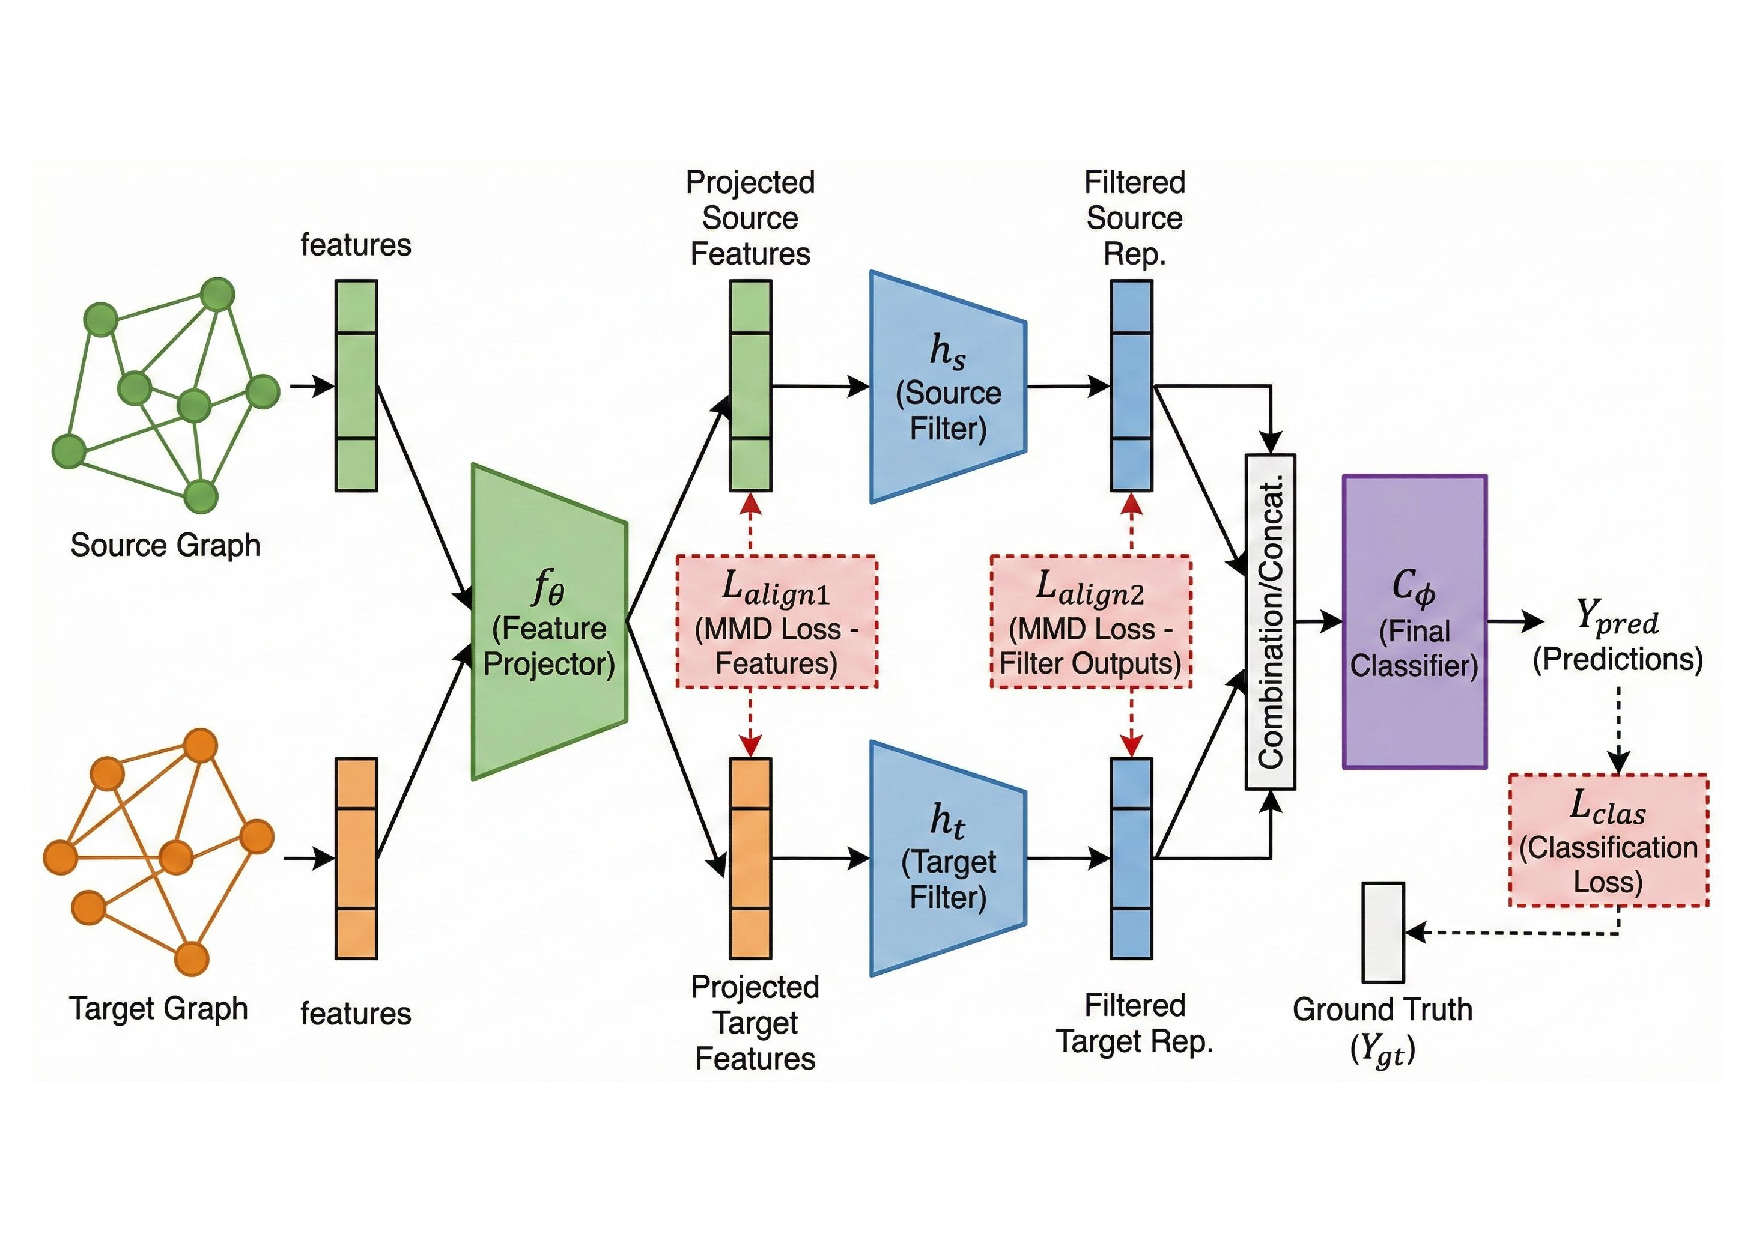
\includegraphics[width=\textwidth]{src/model_figure.pdf}}{\fbox{\rule{0pt}{2.1in}\rule{0.95\textwidth}{0pt}}}
\caption{Overview of \model. A shared encoder produces hidden node representations, while each domain uses its own realized graph filter $\mR_D=S_{\theta_D}(\widehat{\mA}_D)$, reused across layers, to propagate information. Training combines source supervision, Sinkhorn alignment of latent feature distributions, and bootstrap-based alignment of filter responses computed on a common empirical feature support. This directly targets both semantic shift and propagation-induced structural shift without modifying the graph topology.}
\label{fig:opal}
\end{figure}

%%%%%%%%%%%%%%%%%%%%%%%%%%%%%%%%%%%%%%%%%%%%%%%%%%%%%%%%%%%%%%%%%%%%%%
\section{Experiments}

\subsection{Main performance comparison}

We evaluate \model\ on standard UGDA node-classification benchmarks over citation, social, and airport graphs. We report our results mean $\pm$ standard deviation over five seeds and paired significance tests against the strongest recent baselines \cite{pygda}.

\paragraph{Datasets.}
We use ArnetMiner, BlogCatalog, Twitch, and Airport. From Twitch we follow prior work and use the three largest domains: England (EN), Germany (DE), and France (FR).

\paragraph{Baselines.}
The baselines cover embedding-alignment, structure-aware, and propagation/spectral UGDA methods. Concretely, we compare against A2GNN \cite{a2gnn}, AdaGCN \cite{adagcn}, DANE \cite{dane}, DGSDA \cite{dgsda}, GRADE \cite{grade}, JHGDA \cite{jhgda}, KBL \cite{kbl}, PairAlign \cite{pair_align}, SpecReg \cite{specreg}, StruRW \cite{stru_rw}, TDSS \cite{tdss}, and UDAGCN \cite{udagcn}. This set covers the main families discussed in Section 2 and provides a stronger comparison than limiting evaluation to embedding-alignment baselines only.

\paragraph{Implementation details.}
To address reproducibility concerns, the revised variant should report: number of propagation layers $L$, polynomial order $K\in\{2,3,4,5\}$, hidden dimension $d_h$, Sinkhorn regularization $\varepsilon\in\{0.01,0.05,0.1,0.5\}$, and trade-off weights $\lambda_{\mathrm{feat}}$, $\lambda_{\mathrm{filt}}$, and $\lambda_{\mathrm{Lip}}$. Bootstrap probes are resampled at every training iteration. For all datasets, we run experiments for 5 seeds.

\paragraph{Results.}
Table~\ref{table:evaluation} shows kasu
\input{src/eval_table2.tex}

\subsection{Bootstrap probe ablation}

% This experiment isolates the role of the reference distribution used for filter alignment. We compare probes drawn from the pooled feature law, source-only reference probes, target-only reference probes, and a variant without filter alignment. The goal is to verify that aligning realized filters on a common empirical feature support yields better adaptation than comparing them on domain-specific supports.

\subsection{Robustness to structural perturbation}

% This experiment evaluates robustness when the target graph is perturbed by edge rewiring or weight noise. Since the theory identifies a graph perturbation term and an operator-response term, this section studies whether the integral-Lipschitz regularizer improves stability under structural noise.

\subsection{Understanding realized filters as induced propagation graphs}

% A realized graph filter can be viewed as an induced weighted propagation graph. We therefore analyze the learned filters through frequency-response curves, dense matrices, and graph-level summaries such as effective propagation range. The goal is to understand whether the learned filters remain domain-specific while reducing only the harmful part of the structural mismatch.

\subsection{Ablation and hyperparameter study}

% We ablate the feature alignment loss, the reference-based filter alignment loss, and the integral-Lipschitz regularizer. We further study the sensitivity to the number of layers L, polynomial order K, Sinkhorn regularization epsilon, and the trade-off weights in Eq.~\eqref{eq:full_objective_final}. The main questions are which components are necessary and how sensitive the method is to the choice of the filter order.

%%%%%%%%%%%%%%%%%%%%%%%%%%%%%%%%%%%%%%%%%%%%%%%%%%%%%%%%%%%%%%%%%%%%%%
\section{Conclusion}

This paper argues that structural adaptation in UGDA should be formulated at the level of \emph{realized graph filters}. Once the notation is organized around graph shift operators, spectral responses, and realized propagation operators, the key issue becomes clear: even after hidden features are aligned, domain-specific message passing can recreate discrepancy unless the realized filters themselves are controlled. \model\ implements this perspective with a shared encoder, domain-specific filters reused across layers, Sinkhorn feature alignment, and reference-based filter alignment on a common empirical feature support. A lightweight integral-Lipschitz regularizer further stabilizes the learned propagation operators without imposing explicit spectral smoothing. Empirically, the resulting method remains competitive with recent structure-aware UGDA baselines while avoiding graph matching and direct topology modification.

A natural next step is source-free adaptation. Since the filter alignment loss compares realized propagation operators through their responses on feature-supported probes rather than through raw source features, the same principle may remain applicable even when source data are unavailable at adaptation time.

\nocite{*}
\bibliographystyle{splncs04}
\bibliography{mybibliography}

%%%%%%%%%%%%%%%%%%%%%%%%%%%%%%%%%%%%%%%%%%%%%%%%%%%%%%%%%%%%%%%%%%%%%%
\appendix
\section{Appendix: Additional + Proofs}

\subsection{Additional Experiment 1: Distribution shift and performance degradation}
In this experiment, we analyze the relationship between the distribution shift due to domains, and the performance degradation of model trained on source domain and tested on target domain. We use Wasserstein distance to measure the distribution shift, and accuracy drop to measure the performance degradation. We find that there is a positive correlation between the two, which suggests that larger distribution shift leads to more performance degradation. This motivates the need for domain adaptation methods that can reduce the distribution shift and improve the performance on target domain.




\subsection{Proof of Proposition~\ref{prop:propagated_wasserstein}}
\label{app:proof_layer}

\begin{proof}
Let $\pi$ be any coupling between $P_S$ and $P_T$. The pushforward of $\pi$ by $(u,v)\mapsto(\mR_Su,\widetilde{\mR}_Tv)$ is a coupling between $P_S^{\mR}$ and $P_T^{\mR}$. Therefore,
\[
W_1(P_S^{\mR},P_T^{\mR})
\le
\int \|\mR_Su-\widetilde{\mR}_Tv\|_2\, d\pi(u,v).
\]
Add and subtract $\widetilde{\mR}_T u$:
\[
\|\mR_Su-\widetilde{\mR}_Tv\|_2
\le
\|(\mR_S-\widetilde{\mR}_T)u\|_2+\|\widetilde{\mR}_T(u-v)\|_2.
\]
Using $\|\widetilde{\mR}_T(u-v)\|_2\le \|\widetilde{\mR}_T\|_{\mathrm{op}}\|u-v\|_2$ and integrating with respect to $\pi$ yields
\[
W_1(P_S^{\mR},P_T^{\mR})
\le
\mathbb E_{u\sim P_S}\|(\mR_S-\widetilde{\mR}_T)u\|_2
+\|\widetilde{\mR}_T\|_{\mathrm{op}}\int\|u-v\|_2\,d\pi(u,v).
\]
Finally, minimize over all couplings $\pi$ to obtain Eq.~\eqref{eq:propagated_wasserstein}.
\end{proof}

\subsection{Proof of Theorem~\ref{thm:operator_da}}
\label{app:proof_operator_da}

\begin{proof}
Apply the Redko-style OT DA bound at the propagated representation level, i.e., to the pair of distributions $(P_S^{\mR},P_T^{\mR})$. This yields
\[
\epsilon_T(g)
\le
\widehat\epsilon_S(g)
+\sqrt{
\frac{4d}{n_S}\log\frac{en_S}{d}
+
\frac{1}{n_S}\log\frac{1}{\delta}
}
+2C_gW_1(P_S^{\mR},P_T^{\mR})+\omega.
\]
Now invoke Proposition~\ref{prop:propagated_wasserstein}:
\[
W_1(P_S^{\mR},P_T^{\mR})
\le
\mathcal D_{\mathrm{op}}(\mR_S,\widetilde{\mR}_T;P_S)
+
\|\widetilde{\mR}_T\|_{\mathrm{op}}W_1(P_S,P_T).
\]
Substituting this inequality into the OT bound proves Eq.~\eqref{eq:operator_da_bound}.
\end{proof}

\subsection{Proof of Proposition~\ref{prop:coef_ilip}}
\label{app:proof_coefilip}

\begin{proof}
Let $q(\lambda)=\sum_{k=0}^{K_q}a_k\lambda^k$. Then
\[
q'(\lambda)=\sum_{k=1}^{K_q}ka_k\lambda^{k-1}.
\]
Multiplying by $\lambda$ gives
\[
\lambda q'(\lambda)=\sum_{k=1}^{K_q}ka_k\lambda^k.
\]
Hence, for $|\lambda|\le 1$,
\[
|\lambda q'(\lambda)|
\le
\sum_{k=1}^{K_q}k|a_k||\lambda|^k
\le
\sum_{k=1}^{K_q}k|a_k|.
\]
Taking the supremum over $|\lambda|\le 1$ proves Eq.~\eqref{eq:coef_ilip}.
\end{proof}

\end{document}